\chapter{Experiment Result and Analysis}
\label{Chapter4}
\section{Experimental Setting}
\subsection{Evaluation metric}
To test the effectiveness of our algorithms, several evaluation metrics would be used:

\begin{itemize}
	\item $l_1$ norm accuracy 
    \begin{equation}
		l_1(f,g) = \int |f(x)-g(x)|dx
	\end{equation}
	\begin{equation}
		\text{Acc}(f,g) = 1 - \frac{1}{2}l_1(f,g) 
	\end{equation}
    \item Running Speed: Total number of time (second) used for generating posterior density
	
\end{itemize}

Firstly, a common choice for comparing Probability Density Functions if $l_1$ norm


Objective: Use math to find posterior mode of lasso distribution: Given a,b,c
Task: Check if posterior estimate reach 
Metric: Use Posterior TP/FP Rate(Soft thresholding operator) Check if a local parameter mode is close to 0, compared with true parameteer and use this for 
Variable Selection

Expectation: posterior mode sparse, posterior mean not sparse

\subsection{Experimental datasets}
The following bullet points demonstrate the dataset description, which includes the introduction to the purpose of datset, and number of predictos and number of samples respectively.
\begin{itemize}
	
	\item \textbf{Hitters}:
	\begin{itemize}
		\item Type: Baseball statistics dataset
		\item Predictors ($p$): 20, Samples ($n$): 263
		\item Description: Contains baseball player statistics, including performance measures and salary information.
	\end{itemize}
	
	\item \textbf{Kakadu}:
	\begin{itemize}
		\item Type: Environmental dataset
		% ????????
		\item Predictors ($p$): 22, Samples ($n$): 1828
		\item Description: Relates environmental factors to the abundance of amphibians in Kakadu National Park, Australia.
	\end{itemize}
	
	\item \textbf{Bodyfat}:
	\begin{itemize}
		\item Type: Human body measurements dataset
		\item Predictors ($p$): 15, Samples ($n$): 250
		\item Description: Contains measurements of various body parts for a sample of individuals, such as weight, height, and circumferences.
	\end{itemize}
	\item \textbf{Prostate}:
	\begin{itemize}
		\item Type: Medical dataset
		\item Predictors ($p$): 8, Samples ($n$): 97
		\item Description: Prostate cancer data with clinical measurements and Logarithm of Prostate Specific Antigen (lpsa).
	\end{itemize}
	
	\item \textbf{Credit}:
	\begin{itemize}
		\item Type: Credit scoring dataset
		\item Predictors($p$): 11, Samples ($n$): 400
		\item Description: Contains information about loan applicants, such as credit history, employment, and demographics, to assess creditworthiness.
	\end{itemize}
	
	\item \textbf{Eyedata}:
	\begin{itemize}
		\item Type: Medical dataset
		\item Predictors ($p$): 200, Samples ($n$): 120
		\item Description: Contains measurements related to glaucoma patients, such as intraocular pressure and visual acuity, to assess the effectiveness of treatment options.
	\end{itemize}
\end{itemize}

\section{Experimental Result}
\subsection{Approximation Accuracy Result}
\begin{table}[!h]
	\resizebox{\linewidth}{!}{
		\begin{tabular}{|p{3cm}||c| c| c|c|c|c|}
			\hline
			Algorithm  & MCMC  & VB & LG\_Local & LG\_Global \\
			\hline
			Min.   &   100 & 86.8     &  97.3   &   89.3\\
			1st Qu. &  100 & 92.1  &   99.2  &    97.0\\
			Median &  100 & 95.7     &  99.6   &   97.4\\
			Mean  &   100 & 94.2   &  99.3  &    97.1\\
			3rd Qu.&  100 &  97.4     &  99.7  &    99.0\\
			Max.  &   100 & 98.7    &  99.8   &   99.7\\
			Run Time(s) &  453.75  & 0.17  & 0.17  & 0.17 \\
			\hline
	\end{tabular}}
	\caption{Experiment Result on Hitters dataset}
	\label{table:Hitter}
\end{table}
\begin{table}[!h]
	\resizebox{\linewidth}{!}{
		\begin{tabular}{|p{3cm}||c| c| c|c|c|c|}
			\hline
			Algorithm  & MCMC  & VB & LG\_Local & LG\_Global \\
			\hline
			Min.   &  100 &93.2    &   95.9    &  92.2\\
			1st Qu.&  100 & 98.9  &    99.8   &   99.2\\
			Median &  100 & 99.2    &   99.8   &   99.4\\
			Mean   &  100 &  98.6  &    99.4 &     98.8\\
			3rd Qu.&  100 & 99.3  &   99.8 &     99.8\\
			Max.   &  100 & 99.7  &   99.8  &    99.8\\
			Run Time(s) &6696.56 & 0.14 &0.19 & 0.19\\
			\hline
	\end{tabular}}
	\caption{Experiment Result on Kakadu dataset}
	\label{table:Kakadu}
\end{table}
\begin{table}[!h]
	\resizebox{\linewidth}{!}{
		\begin{tabular}{|p{3cm}||c| c|c| c|c|c|c|}
		\hline
		Algorithm  & MCMC  & VB & LG\_Local & LG\_Global \\
		\hline
		Min.   &  100  & 91.3     &   96.3  &     90.7\\
		1st Qu. & 100  & 97.0      &  99.6   &    97.6\\
		Median  &  100  & 98.0    &   99.7  &     98.4\\
		Mean    &  100 &  97.0     &   99.2   &    97.2\\
		3rd Qu.  & 100  &  98.4      &   99.7  &     98.6\\
		Max.    &  100 & 99.3    &   99.7    &   99.7\\
		Run Time(s) &  398.59  & 0.14   & 0.17  & 0.17 \\
		\hline
	\end{tabular}}
	\caption{Experiment Result on bodyfat dataset}
	\label{table:bodyfat}
\end{table}
\begin{table}[!h]
	\resizebox{\linewidth}{!}{
		\begin{tabular}{|p{3cm}||c| c|c| c|c|c|c|}
			\hline
			Algorithm  & MCMC  & VB & LG\_Local & LG\_Global \\
			\hline
			Min.  &   100& 96.9 &    99.5   &   97.4\\
			1st Qu. & 100& 97.2 &    99.5   &   97.9\\
			Median &  100& 97.6  &    99.6   &   98.9\\
			Mean  &   100& 97.5  &    99.6  &    98.7\\
			3rd Qu.&  100& 97.7   &   99.6  &    99.5\\
			Max.   &  100& 98.4  &    99.6  &    99.6\\
			Run Time(s) &  336.31  & 0.11  & 0.12  & 0.12 \\
			\hline
	\end{tabular}}
	\caption{Experiment Result on Prostate dataset}
	\label{table:prostate}
\end{table}
\begin{table}[!h]
	\resizebox{\linewidth}{!}{
		\small
		\begin{tabular}{|p{3cm}||c| c|c| c|c|c|c|}
			\hline
			Algorithm  & MCMC  & VB & LG\_Local & LG\_Global \\
			\hline
			Min.   &  100& 91.8   &   99.5   &   99.3\\
			1st Qu. & 100& 98.3 &    99.7   &   99.5\\
			Median &  100& 99.4   &   99.8   &   99.5\\
			Mean   &  100& 97.9   &   99.7   &   99.6\\
			3rd Qu.&  100 & 99.5   &  99.8   &   99.7\\
			Max.  &   100 & 99.7   &    99.8   &   99.8\\
			Run Time(s) &  359.92  & 0.1  & 0.11  & 0.11 \\
			\hline
	\end{tabular}}
	\caption{Experiment Result on Credit dataset}
	\label{table:Credit}
\end{table}
\begin{table}[!h]
	\resizebox{\linewidth}{!}{
		\small
		\begin{tabular}{|p{3cm}||c| c|c| c|c|c|c|}
			\hline
			Algorithm  & MCMC  & VB & LG\_Local & LG\_Global \\
			\hline
			Min.    & 100 & 78.4   &   97.3   &   86.1\\
			1st Qu. & 100 & 86.9   &   98.6   &   90.4\\
			Median &  100 & 90.3   &   98.7  &    91.3\\
			Mean   & 100 & 88.9  &   98.7  &    91.8\\
			3rd Qu. & 100 &91.2    &  98.8   &   92.3\\
			Max.   &  100 &93.1  &   99.1  &    99.2\\
			Run Time(s) &  18144.7  & 1.21  & 1.72  & 1.72 \\
			\hline
	\end{tabular}}
	\caption{Experiment Result on Eyedata dataset}
	\label{table:Eyedata}
\end{table}

\subsection{Approximation Density Visualization}

\begin{figure}[h]
	\centering
	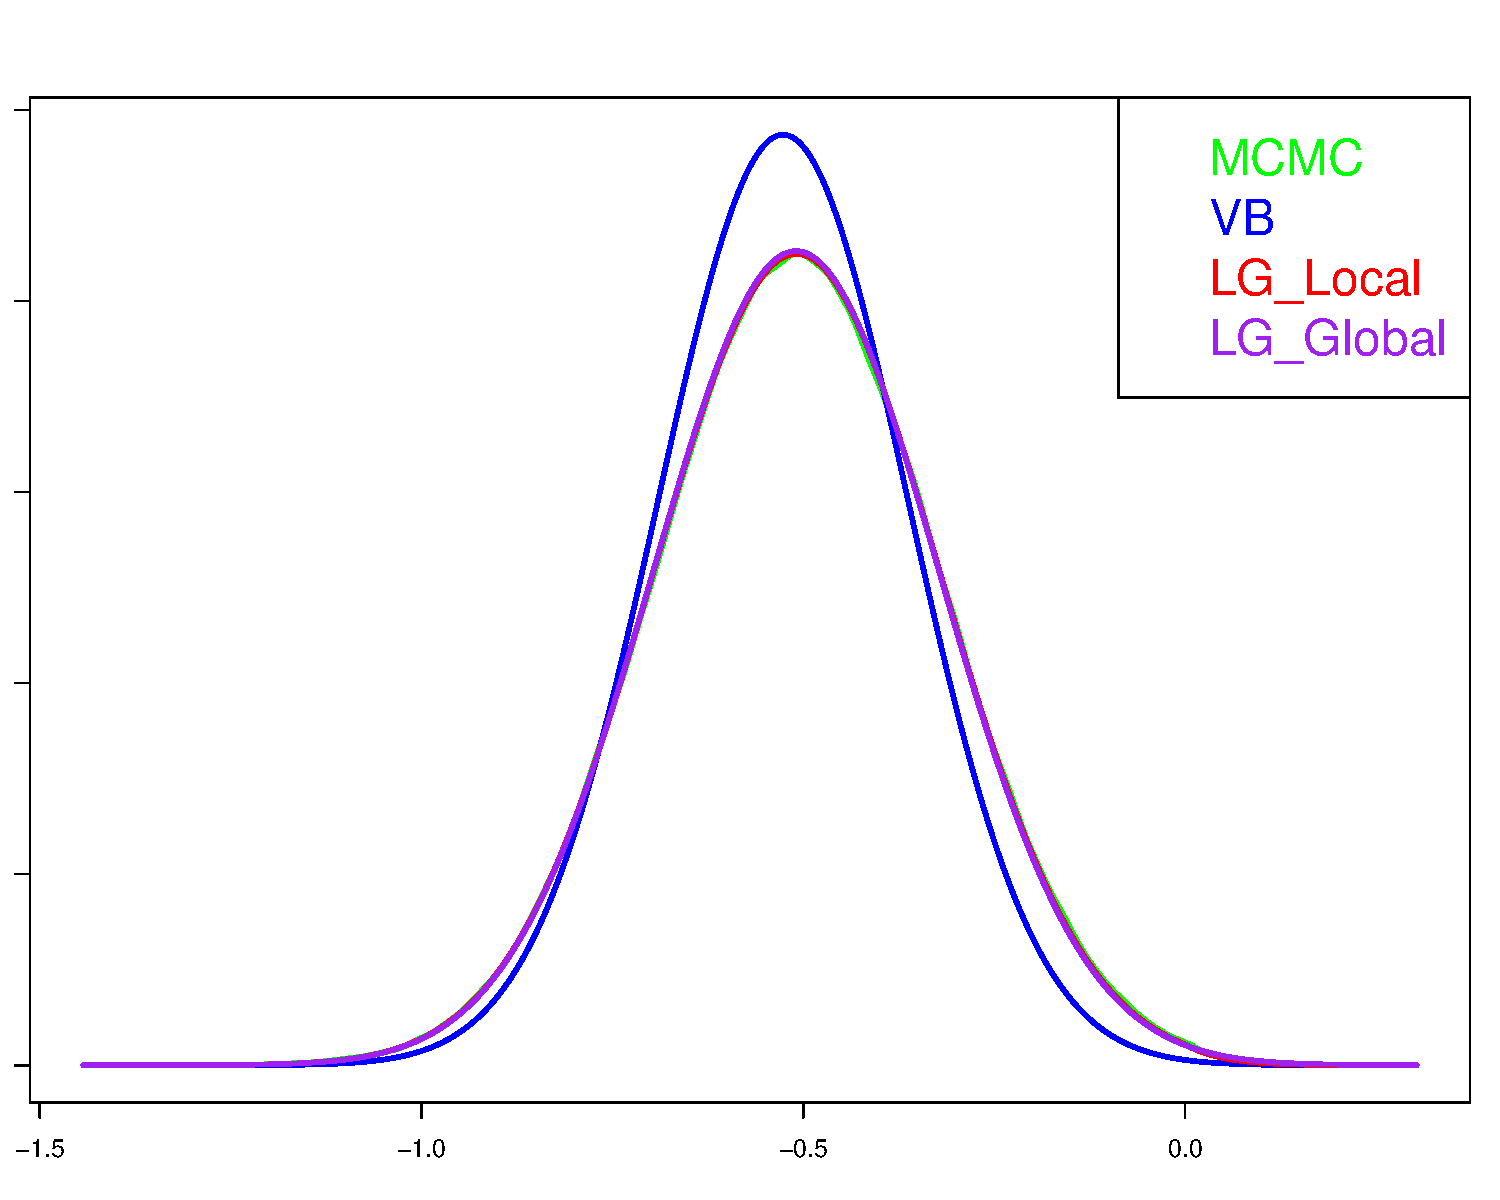
\includegraphics[page = 1, width=\linewidth,keepaspectratio]{lasso_densities_Hitters.pdf}
	\caption{Part of Approximation Density for Hitters dataset}
	\label{fig:hitters1}
\end{figure}
	
\begin{figure}[h]
	\centering
	\includegraphics[page = 2, width=\linewidth,keepaspectratio]{lasso_densities_Hitters.pdf}
	\caption{Part of Approximation Density for Hitters dataset}
	\label{fig:hitters2}
\end{figure}



